% Options for packages loaded elsewhere
\PassOptionsToPackage{unicode}{hyperref}
\PassOptionsToPackage{hyphens}{url}
%
\documentclass[
  12pt,
]{article}
\usepackage{amsmath,amssymb}
\usepackage{lmodern}
\usepackage{ifxetex,ifluatex}
\ifnum 0\ifxetex 1\fi\ifluatex 1\fi=0 % if pdftex
  \usepackage[T1]{fontenc}
  \usepackage[utf8]{inputenc}
  \usepackage{textcomp} % provide euro and other symbols
\else % if luatex or xetex
  \usepackage{unicode-math}
  \defaultfontfeatures{Scale=MatchLowercase}
  \defaultfontfeatures[\rmfamily]{Ligatures=TeX,Scale=1}
\fi
% Use upquote if available, for straight quotes in verbatim environments
\IfFileExists{upquote.sty}{\usepackage{upquote}}{}
\IfFileExists{microtype.sty}{% use microtype if available
  \usepackage[]{microtype}
  \UseMicrotypeSet[protrusion]{basicmath} % disable protrusion for tt fonts
}{}
\usepackage{xcolor}
\IfFileExists{xurl.sty}{\usepackage{xurl}}{} % add URL line breaks if available
\IfFileExists{bookmark.sty}{\usepackage{bookmark}}{\usepackage{hyperref}}
\hypersetup{
  pdftitle={Analytical choices for analyzing multidimensional behavior - Many analysts test hypotheses about human speech.},
  pdfkeywords={crowdsourcing science, data analysis, scientific transparency, speech, acoustic analysis},
  hidelinks,
  pdfcreator={LaTeX via pandoc}}
\urlstyle{same} % disable monospaced font for URLs
\usepackage[margin=4cm]{geometry}
\usepackage{longtable,booktabs,array}
\usepackage{calc} % for calculating minipage widths
% Correct order of tables after \paragraph or \subparagraph
\usepackage{etoolbox}
\makeatletter
\patchcmd\longtable{\par}{\if@noskipsec\mbox{}\fi\par}{}{}
\makeatother
% Allow footnotes in longtable head/foot
\IfFileExists{footnotehyper.sty}{\usepackage{footnotehyper}}{\usepackage{footnote}}
\makesavenoteenv{longtable}
\usepackage{graphicx}
\makeatletter
\def\maxwidth{\ifdim\Gin@nat@width>\linewidth\linewidth\else\Gin@nat@width\fi}
\def\maxheight{\ifdim\Gin@nat@height>\textheight\textheight\else\Gin@nat@height\fi}
\makeatother
% Scale images if necessary, so that they will not overflow the page
% margins by default, and it is still possible to overwrite the defaults
% using explicit options in \includegraphics[width, height, ...]{}
\setkeys{Gin}{width=\maxwidth,height=\maxheight,keepaspectratio}
% Set default figure placement to htbp
\makeatletter
\def\fps@figure{htbp}
\makeatother
\setlength{\emergencystretch}{3em} % prevent overfull lines
\providecommand{\tightlist}{%
  \setlength{\itemsep}{0pt}\setlength{\parskip}{0pt}}
\setcounter{secnumdepth}{5}
\usepackage{cleveref}
\setlength{\marginparwidth}{2cm}
\usepackage[todonotes={textsize=tiny}]{changes}
\definechangesauthor[name={Stefano Coretta}, color=red]{SC}
\definechangesauthor[name={Timo Röttger}, color=blue]{TR}
\definechangesauthor[name={Joseph Casillas}, color=orange]{JC}
\ifluatex
  \usepackage{selnolig}  % disable illegal ligatures
\fi
\newlength{\cslhangindent}
\setlength{\cslhangindent}{1.5em}
\newlength{\csllabelwidth}
\setlength{\csllabelwidth}{3em}
\newenvironment{CSLReferences}[2] % #1 hanging-ident, #2 entry spacing
 {% don't indent paragraphs
  \setlength{\parindent}{0pt}
  % turn on hanging indent if param 1 is 1
  \ifodd #1 \everypar{\setlength{\hangindent}{\cslhangindent}}\ignorespaces\fi
  % set entry spacing
  \ifnum #2 > 0
  \setlength{\parskip}{#2\baselineskip}
  \fi
 }%
 {}
\usepackage{calc}
\newcommand{\CSLBlock}[1]{#1\hfill\break}
\newcommand{\CSLLeftMargin}[1]{\parbox[t]{\csllabelwidth}{#1}}
\newcommand{\CSLRightInline}[1]{\parbox[t]{\linewidth - \csllabelwidth}{#1}\break}
\newcommand{\CSLIndent}[1]{\hspace{\cslhangindent}#1}

\title{Analytical choices for analyzing multidimensional behavior - Many analysts test hypotheses about human speech.}
\author{true \and true \and true \and true}
\date{}

\begin{document}
\maketitle
\begin{abstract}
One or two sentences providing a \textbf{basic introduction} to the field, comprehensible to a scientist in any discipline.

Two to three sentences of \textbf{more detailed background}, comprehensible to scientists in related disciplines.

One sentence clearly stating the \textbf{general problem} being addressed by this particular study.

One sentence summarizing the main result (with the words ``\textbf{here we show}'' or their equivalent).

Two or three sentences explaining what the \textbf{main result} reveals in direct comparison to what was thought to be the case previously, or how the main result adds to previous knowledge.

One or two sentences to put the results into a more \textbf{general context}.

Two or three sentences to provide a \textbf{broader perspective}, readily comprehensible to a scientist in any discipline.
\end{abstract}

{
\setcounter{tocdepth}{2}
\tableofcontents
}
\hypertarget{introduction}{%
\section{Introduction}\label{introduction}}

In order to effectively accumulate knowledge, science needs (i) to produce data that can be replicated using the original methods and (ii) to arrive at robust conclusions substantiated by the data.
In recent coordinated efforts to replicate published findings, the scientific disciplines have uncovered surprisingly low success rates in replication attempts (e.g., Open Science Collaboration 2015; Camerer et al. 2018) leading to what is now referred to as the \emph{replication crisis}.
Beyond the difficulties of replicating scientific findings, a growing body of evidence suggests that the theoretical conclusions drawn from data are often variable even when researchers have access to reliable data (\highlight{REFS}).
The latter situation has been referred to as the \emph{inference crisis} (Rotello, Heit, and Dubé 2015; Jeffrey J. Starns et al. 2019b) and is, among other things, rooted in the inherent flexibility of data analysis (often referred to as researcher degrees of freedom: Simmons, Nelson, and Simonsohn 2011; Gelman and Loken 2014).
Data analysis involves many different steps, such as inspecting, organizing, transforming, and modeling the data, to name a few.
Along the way, different methodological and analytical choices need to be made, all of which may influence the final interpretation of the data.
These researcher degrees of freedom are both a blessing and a curse.

They are a blessing because they afford us the opportunity to look at nature from different angles, which, in turn, allows us to make important discoveries and generate new hypothesis (e.g., Box 1976; Tukey 1977; De Groot 2014).
They are a curse because idiosyncratic choices can lead to categorically different interpretations, which eventually find their way into the publication record where they are taken for granted (Simmons, Nelson, and Simonsohn 2011).
Recent projects have shown that the variability between different data analysts is vast.
This variability can lead independent researchers to draw different conclusions about the same data set as demonstrated by several projects crowd-sourcing analysis strategies (e.g., Silberzahn et al. 2018; Jeffrey J. Starns et al. 2019b; Botvinik-Nezer et al. 2020b).
These projects, however, might still underestimate the extent to which analysts vary because data analysis is not merely restricted to statistical inference.
Human behavior is complex and offers many ways to be translated into numbers.
This is particularly true for fields that draw conclusions about human behavior and cognition from multidimensional data like audio or video data.
In fields working on human speech production, for example, researchers need to make numerous decisions about what to measure and how to measure it.
This is not trivial, given the temporal extension of the acoustic signal and its complex structural composition.
Not only can decisions about measuring the signal influence downstream decisions about statistical modeling, but statistical results or modeling issues can also lead researchers to go back and revise earlier decisions about the measuring process itself.

In this article, we investigate the variability in analytic choices when many analyst teams analyze the same speech production data, a process that involves both decisions regarding the operationalization of a complex observed signal and decisions regarding the statistical modeling.
Specifically, we report the impact of the analytic pipeline on research results obtained by XX teams who gained access to the same set of acoustic recordings in order to answer the same research question.

\hypertarget{researcher-degrees-of-freedom}{%
\subsection{Researcher degrees of freedom}\label{researcher-degrees-of-freedom}}

Data analysis comes with many decisions like how to measure a given phenomenon or behavior, what data to submit to statistical modeling and which to exclude in the final analysis, or what inferential decision procedure to apply.
\highlight[id=JC, comment = {I'd probably drop this. When we make unspecified decisions during data analysis we can stumble upon spurious results (most likely) as well as real results (less likely, still possible)... in other words it might not all be error... the issue is that we won't know the difference}]{However, if these decisions} during data analysis are not specified in advance, we might stumble upon seemingly meaningful patterns in the data that are merely statistical flukes.\comment[id=TR]{But isn't the human bias the major issue in statistical misinterpretation? (It also leads naturally to the next paragraph.)}
This can be problematic because humans show cognitive biases that can lead to erroneous inferences.
Humans filter the world in irrational ways (e.g., Tversky and Kahneman 1974), seeing coherent patterns in randomness (Brugger 2001), convincing themselves of the validity of prior expectations ({``I knew it,''} Nickerson 1998), and perceiving events as being plausible in hindsight ({``I knew it all along,''} Fischhoff 1975).
\comment[id=JC]{If helpful we could also give a concrete common example here, like regarding forecasting the weather or something}
\comment[id=TR]{Generally a good idea, but I'd say we keep it crisp at that point. The take-home here is: Humans are biased.}
In connection with an academic incentive system that rewards certain discovery processes more than others (Sterling 1959; Koole and Lakens 2012), we often find ourselves exploring many possible analytical pipelines, but only reporting a select few.
This issue is particularly amplified in fields in which the raw data lend themselves to many possible ways to measure (Roettger 2019).
Combined with a wide variety of methodological and theoretical traditions as well as varying levels of statistical training across subfields, the inherent flexibility of data analysis might lead to a vast plurality of analytic approaches that can lead to different scientific conclusions.
Consequently, there might be many published papers that present overconfident interpretations of their data based on idiosyncratic analytic strategies (e.g., Simmons, Nelson, and Simonsohn 2011; Gelman and Loken 2014).
These interpretations are either associated with an unknown amount of uncertainty or lend themselves to alternative interpretation if analyzed differently.
However, instead of being critically evaluated, scientific results often remain unchallenged in the publication record.
Despite recent efforts to improve transparency and reproducibility (REFS) and freely available and accessible infrastructures such as provided by the Open Science Framework (osf.io, ADD), critical re-analyses of published analytic strategies are still not very common because data sharing remains rare (Jelte M. Wicherts et al. 2006).

While this issue has been widely discussed both from a conceptual point of view (Simmons, Nelson, and Simonsohn 2011; Wagenmakers et al. 2012; Nosek and Lakens 2014) and its application in individual scientific fields (e.g.~Wichert et al.~2015, Charles et al.~2019, Roettger 2019), there are still many unknowns regarding the extent of analytical plurality in practice.
Recent collaborative attempts have started to shed light on how different analysts tackle the same data set and have revealed a large amount of variability.

\hypertarget{crowdsourcing-alternative-analyses}{%
\subsection{Crowdsourcing alternative analyses}\label{crowdsourcing-alternative-analyses}}

In a collaborative effort, Silberzahn et al. (2018) let twenty-nine independent analysis teams address the same research hypothesis.
Analytical approaches and consequently the results varied widely between teams.
Sixty-nine percent of the teams found support for the hypothesis, and 31\% did not.
Out of the 29 analytical strategies, there were 21 unique combinations of covariates.
Importantly, the observed variability was neither predicted by the team's preconceptions about the phenomenon under investigation nor by peer ratings of the quality of their analyses.
The authors results suggest that analytic plurality is a fact of life and not driven by different levels of expertise or bias.

Similar crowd-sourced studies recruiting independent analyst teams showed similar results.
Both Dutilh et al. (2019) ad Jeffrey J. Starns et al. (2019a) investigated analysts choices when inferring theoretical constructs based on the same data set using computational models.
Both studies reveal vastly different modeling strategies, even though scientific conclusions were similar across analysis teams (see also Parker et al.~(accepted) on analytical flexibility in ecology and Botvinik-Nezer et al. 2020a on neuroimaging data).
Bastiaansen et al. (2020) crowdsourced clinical recommendations based on data analysis of an individual patient.
Results suggests that analysis team differed substantially regarding decisions related to both the statistical analysis of the data set and the theoretical rationale behind interpreting the statistical results, indicating that there are multiple layers for degrees of freedom that interact with each other.

While these projects show a large degree of analytical flexibility with impactful consequences, they dealt with flexibility in inferential or computational modeling.
In these studies the data sets were fixed and data collection or measurement could not be changed.\comment[id=JC]{any particular reason to favor data table over data set?}\comment[id=TR]{I think my reasoning was data set can be data table or raw data. Data table is the numerical derivation of the raw data. Maybe not a useful distinction?}

However, in many fields the primary raw data are complex signals that need to be operationalized in light of the research question.
This is especially true in the social sciences, where the subject of investigation corresponds to observable and unobservable human behavior.
Decisions about how to measure a theoretical construct related to such behavior or its underlying cognitive processes might interact with downstream decisions about statistical modeling and vice versa.
For example, Flake and Fried (2020) discuss the cascading impact different practices can have on several components of psychometric research.
The authors highlight, among others, the following degrees of freedom in the choice and development of measures: definition of the theoretical construct, justification of the selected measure, description of the measure and of how it maps onto the construct, response coding and related transformations, and post-hoc modifications to the chosen measure.
Taken together, these aspects alone exponentially increase the combinations of possible analytical choices, and hence flexibility in research outcomes.

In those social sciences concerned with communication, human behaviour is sometimes measured as a complex visual or acoustic signal.
This added complexity introduces further fork junctions in the research pipe-line, thus increasing yet again analytical flexibility.
The present study looks at experimentally elicited speech data to understand how this flexibility manifests itself in a scenario where complex decision procedures are involved in the operationalization and measuring of complex signals.

\hypertarget{s:operspeech}{%
\subsection{Operationalizing speech}\label{s:operspeech}}

Research on speech is at the heart of the cognitive sciences, informing psychological models of language, categorization, and memory, guiding methods for diagnosis and therapy of speech disorders, and facilitating advancement in automatic speech recognition and speech synthesis.
One major challenge in the speech sciences is the mapping between communicative intentions (the unobserved behavior) and their physical manifestation (the observed behaviour).

Speech is a complex signal that is characterized by structurally different acoustic landmarks distributed throughout different temporal domains.
Thus, choosing how to measure a phenomenon of interest is an important and non-trivial analytical decision.
Take for example the following sentence in (1).

\begin{enumerate}
\def\labelenumi{(\arabic{enumi})}
\tightlist
\item
  ``I can't bear another meeting on Zoom.''
\end{enumerate}

Depending on the speaker's intention, this sentence can be said in different ways.
If, for instance, the speaker is exhausted by all their meetings, the speaker might acoustically highlight the word \emph{another} or \emph{meeting}.
If, on the other hand, the speaker is just tired of video conferences, they might acoustically highlight the word \emph{Zoom}.

If we decide to compare the speech signal associated with these two intentions, how can we quantify the difference between them?
Given their physical manifestation (speech), what do we measure and how do we measure it?
Because of the continuous and transient nature of speech, identifying speech parameters and temporal domains within which to measure those parameters becomes a non-trivial task.
Utterances stretch over hundreds of milliseconds and contain several levels of linguistically relevant units such as phrases, words, syllables, and individual sounds.
The researcher is thus confronted with a considerable number of parameters and combinations thereof to choose from.

Speech categories are inherently multidimensional and dynamic: they consist of a cluster of parameters that are modulated over time.
The acoustic parameters of one category are usually asynchronous, i.e.~they appear at different time points in the unfolding signal, and overlap with parameters of other categories {[}e.g., Jongman, Wayland, and Wong (2000); Lisker (1986); Summerfield, 1984; Winter (2014){]}.
A classical example is the distinction between voiced and voiceless stops in English (i.e.~/b/ and /p/ in \emph{bear} vs \emph{pear}).
This voiced/voiceless contrast is manifested by many acoustic features which can differ depending on several factors, such as position of the consonant in the word and surrounding sounds (Lisker 1977).
Furthermore, correlates of the contrast can even be found away from the consonant, in temporally distant speech units.
For example, the initial /l/ of the English words \emph{led} and \emph{let} is affected by the voicing of the final consonant (/t, d/) (Hawkins and Nguyen 2004).

The multiplicity of phonetic cues grows exponentially if we look at larger temporal domains as is the case for suprasegmental aspects of speech.
For example, studies investigating acoustic correlates of word stress (e.g.~the difference between \emph{insíght} and \emph{íncite}) have been using a wide variety of measurements, including temporal characteristics (duration of certain segments or sub-segmental intervals), spectral characteristics (intensity, formants, and spectral tilt), and measurements related to fundamental frequency (f0) (e.g., Gordon and Roettger 2017).
Moving onto the expression of higher-level functions like information structure and discourse pragmatics, relevant acoustic cues can be distributed throughout even larger domains, such as phrases and whole utterances (e.g., Ladd 2008).
Differences in position, shape, and alignment of pitch modulations over multiple locations within a sentence are correlated with differences in discourse functions (e.g.~Niebuhr et al., 2011).
The latter can also be expressed by global vs local pitch modulations (Van Heuven et al. 2002), as well as acoustic information within the temporal or spectral domain (e.g., Van Heuven and Van Zanten 2005).
Extra-linguistic information, like speaker's intentions, levels of arousal or social identity, are also conveyed by broad-domain parameters, such as voice quality, rhythm, and pitch (Foulkes and Docherty 2006; Ogden 2004; White, Payne, and Mattys 2009).

When testing hypotheses on speech production data, researchers are faced with many choices and possibilities.
The larger the functional domain (e.g.~segments vs words vs utterances), the higher the number of conceivable operationalizations.
For example, several decisions have to be made when comparing the two realization of the sentence in (1), one of which is intended to signal emphasis on \emph{another} and one of which emphasizes \emph{zoom}.

(2a) I can't bear \emph{ANOTHER} meeting on zoom.

(2b) I can't bear another meeting on \emph{ZOOM}.

Do we compare only the word \emph{another} in (2a) and (2b), or also the word \emph{zoom}?
Do we measure utterance-wide acoustic profiles, whole words, or just the stressed syllables?
Do we average across the chosen time domain or do we measure a specific point in time?
Do we measure fundamental frequency, intensity, something else?

When looking at phrase-level temporal domains, the number of possible analytical pipelines quickly explodes.
This plurality of analytical paths is illustrated in Figure \ref{fig:forkingPaths}.
When comparing two utterance such as (2a) and (2b), there are many things to consider.
Even if we have decided to compare fundamental frequency (f0) of only the word \emph{another} across the two utterances, there are still many choices to be made, all of which need to be justified.
For example, we could measure f0 at specific points in time like the onset of the window, the offset, or the midpoint.
We could also measure the value or time of the minimum or maximum f0 value.
We could summarise f0 across the entire window and extract the mean, median or standard deviation of f0.
And the garden of forking paths does not stop here.
In \highlight[id=SC, comment = {The figure text is quite small. Probably better to change to a longer rather then wider layout.}]{Figure} \ref{fig:forkingPaths}, we went with a specific option to automatically calculate f0, INSERT SOME EXAMPLES OF PITCH TRACKING OPTIONS.\comment{add examples of pitch tracking options}
Moreover, knowing that the signals and the measures thereof can be noisy, we could smooth these using one algorithm and degree over others, or remove values that substantially deviate from surrounding values or expectations, either manually or automatically, and so on.



\begin{figure}
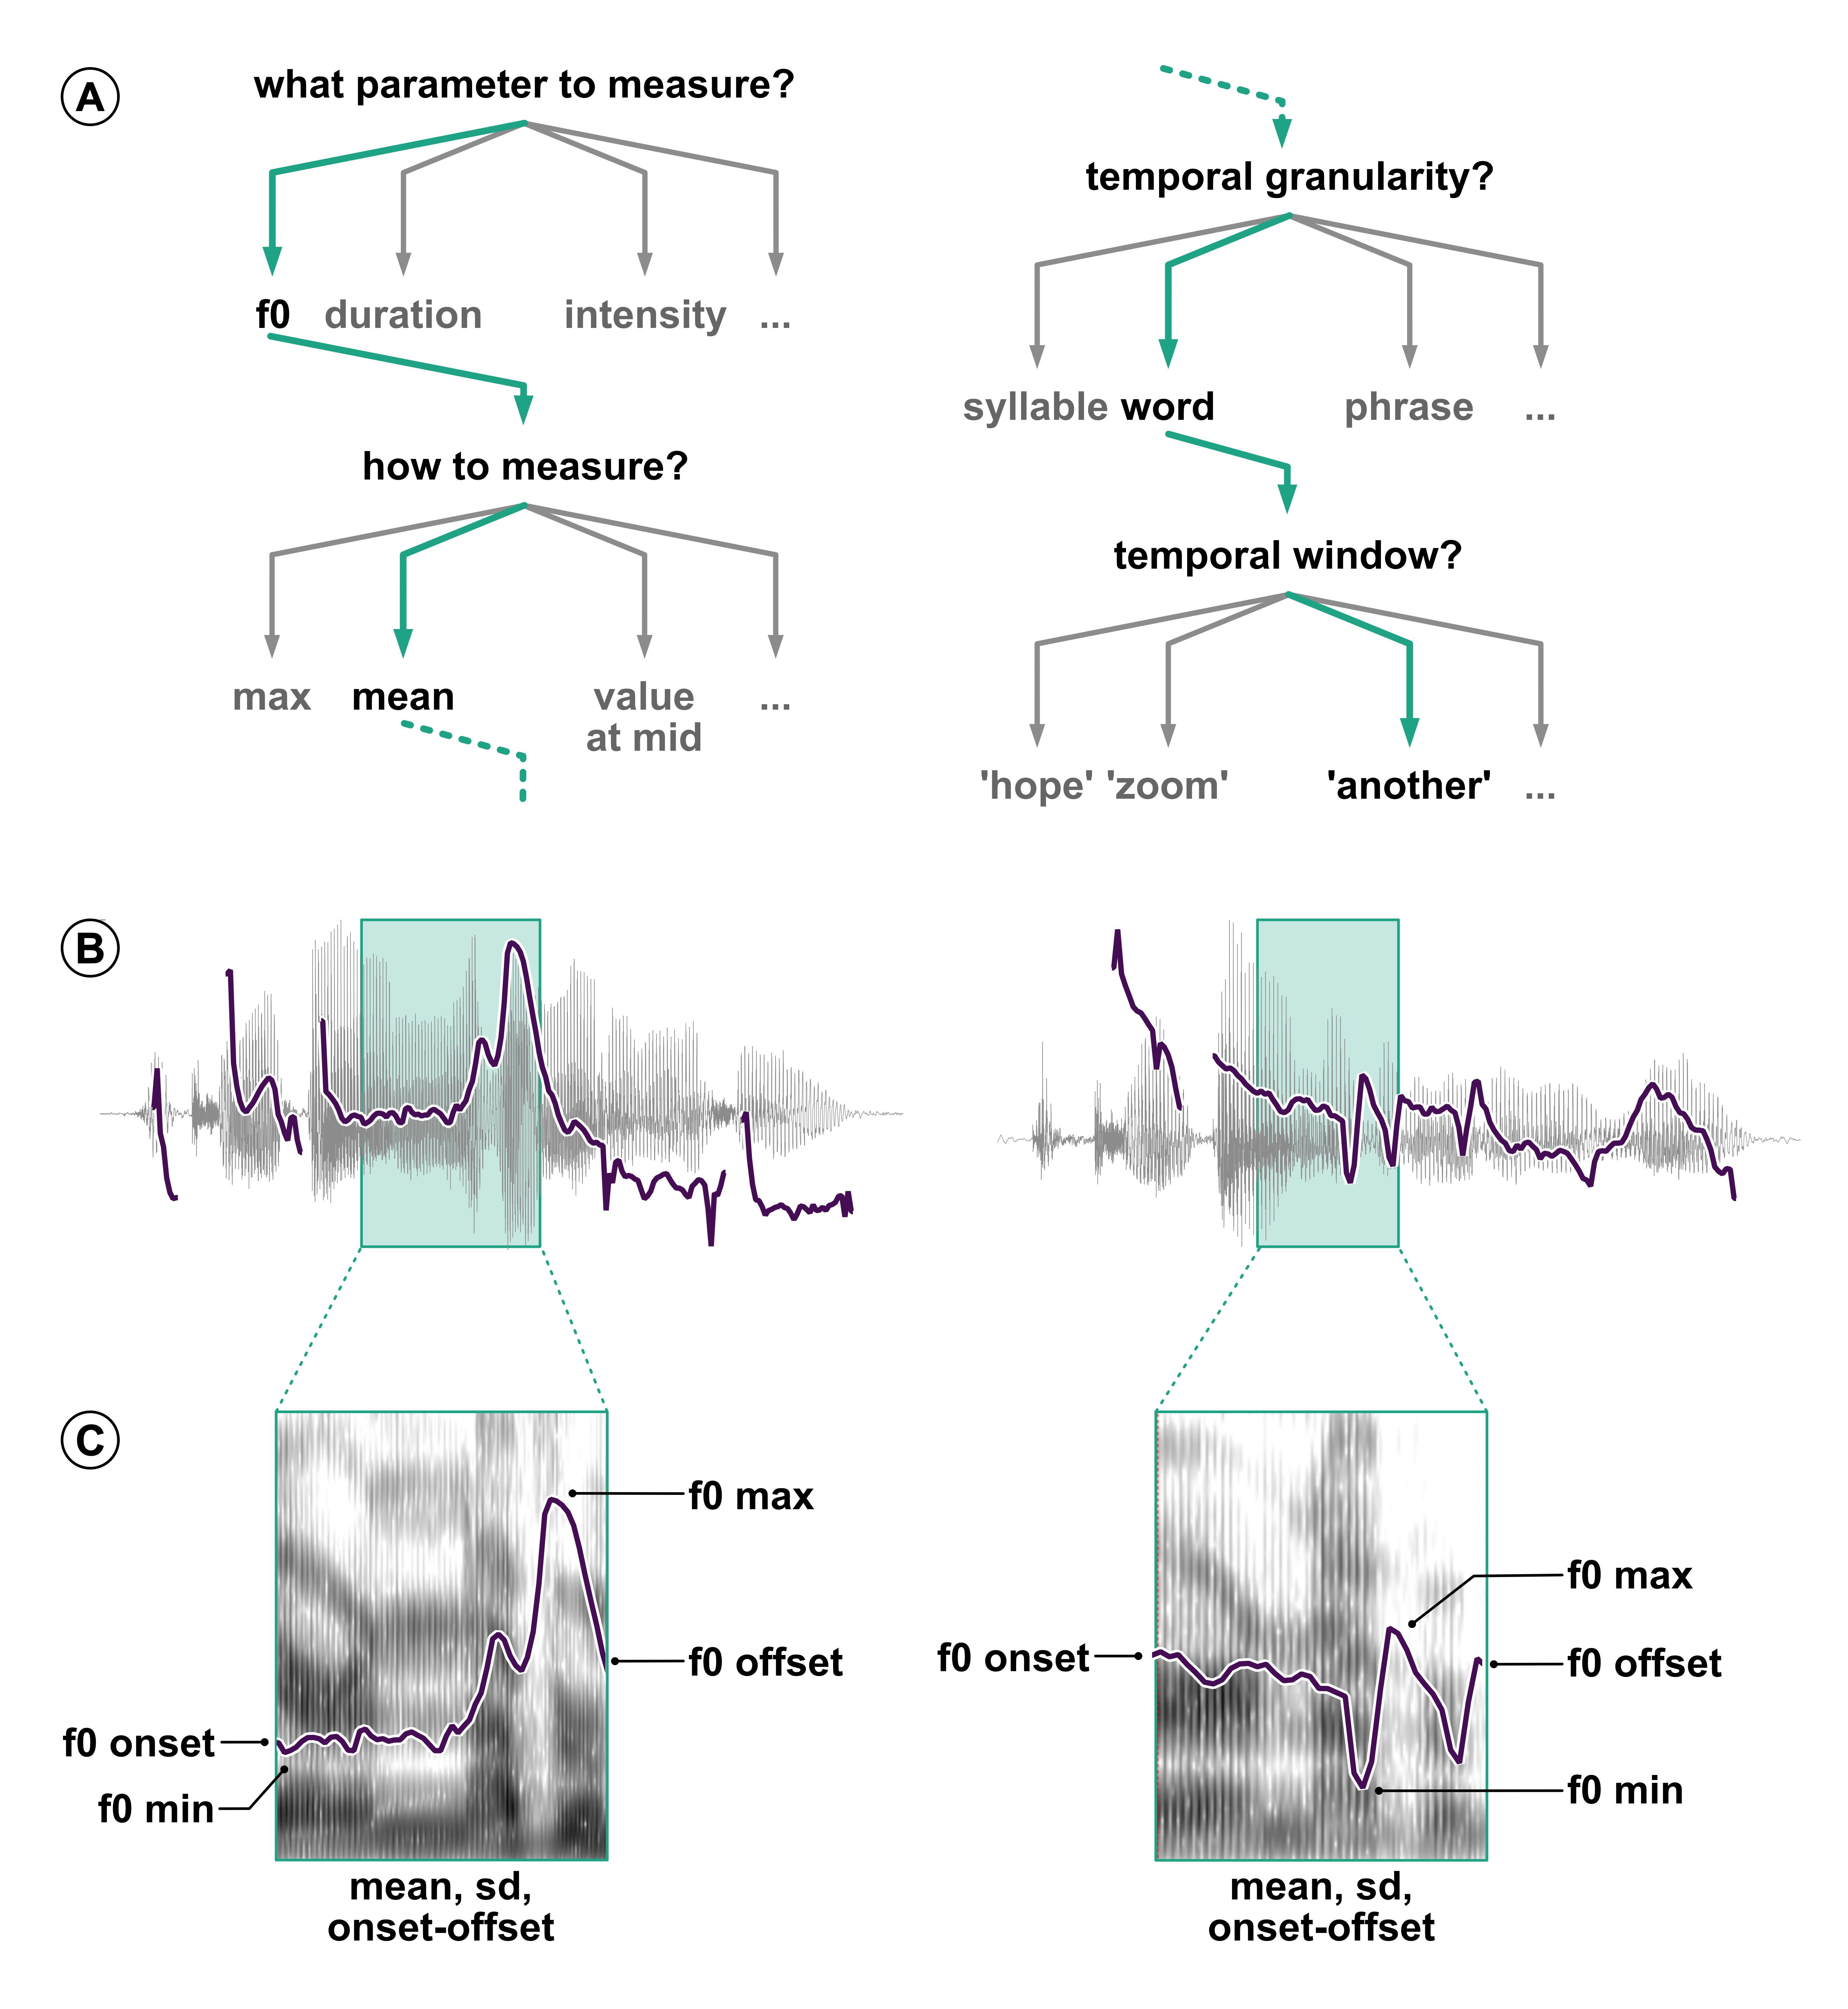
\includegraphics[width=1\linewidth]{/Users/ste/repos/many_analyses/figs/ForkingPaths} \caption{Illustrations of the analytical flexibility associated with acoustic analyses. (A) an example of multiple possible and justifiable decisions when comparing to utterances; (B) waveform and fundamental frequency (f0) track of two instances of utterances 2a and 2b. The words ``another is highlighted by the green box''; (C) spectrogram and f0 track of the word another, exemplifying different operationalizations of differences in pitch.}\label{fig:forkingPaths}
\end{figure}

These decisions are usually made prior to any statistical analysis, but are at times revised a posteriori (i.e.~after data collection and/or preliminary analyses) in light of unforeseen or surprising outcomes.
These myriads of possible decisions are exponentiated by researcher degrees of freedom related to statistical analysis (e.g. Jelte M. Wicherts et al. 2016).
Even the analysis of a single measure can be approached via an ever-increasing range of different statistical models (\highlight{REFs}).
The present paper probes this garden of forking paths in the analysis of speech.
To assess the variability in data analysis pipelines across independent researchers, we provided XX analytical teams with an experimentally elicited speech corpus and asked them to investigate acoustic differences related to a functional contrast that might be manifested across the whole utterance.\comment[id=SC]{This needs a smother transition.}

\hypertarget{the-data-set-the-acoustic-properties-of-redundant-modifiers}{%
\subsection{The data set: The acoustic properties of redundant modifiers}\label{the-data-set-the-acoustic-properties-of-redundant-modifiers}}

The data set given to the analysis teams comes from a study that investigated whether speakers acoustically modify utterances to signal typicality of noun/adjective combinations in referring expressions such as \emph{a blue banana} (atypical) vs \emph{a yellow banana} (typical).
Referring is one of the most basic and prevalent uses of language and one of the most widely researched areas in language science.
It is an open question how speakers choose a referring expression when they want to refer to a specific entity like a banana.
The context within which an entity occurs (i.e., with other non-fruits, other fruits, or other bananas) plays a large part in determining the choice of referring expressions.
Generally, speakers aim to be as informative as possible to uniquely establish reference to the intended object, but they are also resource-efficient in that they avoid redundancy (Grice 1975).
Thus one would expect the use of a modifier, for example, only if it is necessary for disambiguation.
For instance, one might use the adjective \emph{yellow} to describe a banana in a situation in which there is a yellow and a less ripe green banana available, but not when there is only one banana to begin with.

Despite this coherent idea that speakers are both rational and efficient, there is much evidence that speakers are often over-informative: Speakers use referring expressions that are more specific than strictly necessary for the unambiguous identification of the intended referent (Sedivy 2003; Westerbeek, Koolen, and Maes 2015; Rubio-Fernández 2016), which has been argued to facilitate object identification and making communication between speakers and listeners more efficient (Arts et al. 2011; Paraboni, Van Deemter, and Masthoff 2007; Rubio-Fernández 2016).
Recent findings suggest that the utility of a referring expression depends on how good it is for a listener (compared to other referring expressions) to identify a target object.
For example, Degen et al. (2020) showed that modifiers that are less typical for a given referent (e.g.~a blue banana) are more likely to be used in an over-informative scenario (e.g.~when there is just one banana).
This account, however, has mainly focused on content selection (Gatt et al. 2013), i.e.~whether a certain referential expression is chosen or not, ignoring the fact that speech communication is much richer.

Even looking at morphosyntactically identical expressions, speakers can modulate these via suprasegmental acoustic properties like temporal and spectral modifications of the segments involved (e.g., Ladd 2008).
Most prominently, languages use intonation to signal discourse relationships between referents (among other functions).
Intonation marks discourse-relevant referents for being new or given information to guide the listeners' interpretation of incoming messages.
In many languages, speakers can use particular pitch movements to signal whether a referent has already been mentioned and is therefore referred back to, or a referent is newly introduced into the discourse.
Many languages use intonation in order to signal if a referent is contrasting with one or more alternatives that are relevant to the current discourse.
Content selection aside, in a scenario in which a speaker wants to refer to a banana when there is also a pear on the table, the speaker would most likely produce a high rising pitch accent on \emph{banana} to indicate the contrastive nature of the noun.
In a scenario in which the speaker wants to refer to a yellow banana when there is also a less ripe green banana on the table, the speaker would most likely produce a high rising pitch accent on \emph{yellow} to indicate the contrastive nature of the modifier.
In addition to a pitch accent, elements that are new and/or contrastive are often produced with additional suprasegmental prominence, i.e.~segments are hyperarticulated, resulting in longer, louder and more clearly articulated acoustic targets.

To answer the question of whether speakers modify speech to signal atypical referents, thirty native German speakers were recorded in a speech production study while interacting with a confederate (one of the experimenters).
The participants had to verbally instruct the confederate to select a specified target object out of four object presented on a screen.
The subject and confederate were seated at the opposite sides of a table, each facing one of two mirrored computer screens.
The participant and the experimenter could not see each other nor each others' screens.
After a familiarisation phase (see XXX), the subject first saw four colored objects in the top left, top right, bottom left, and bottom right corners of the screen.
One of the objects served as the target, another as the competitor, and the remaining two objects served as distractors.
Objects were referred to using noun phrases consisting of an adjective modifier denoting color and a modified object (e.g.~\emph{Gelbe Zitrone} `yellow lemon,' \emph{Rote Gurke} `red cucumber,' \emph{Rote Socken} `red socks').

In the center of the screen, a black cube was displayed, which could be moved by the experimenter.
The participant would read a sentence prompt out loud (\emph{Du sollst den Würfel auf der ablegen} `You have to put the cube on top of the ') to instruct the experimenter to drag the cube on top of one of the four depicted objects (the \emph{competitor}) using the mouse.
After the experimenter had moved the cube as instructed, the subject would read another sentence prompt (\emph{Und jetzt sollst du den Würfel auf der ablegen} `And now, you have to put the cube on top of the ') instructing the experimenter to move the cube on top of a different object (the \emph{target}).
The audio of this second utterance in the trial was recorded.

The two sentence prompts were used to create a focus contrast between the competitor and the target object.
If the competitor and target objects differed but their color did not (e.g.~\emph{yellow banana} vs \emph{yellow tomato}), the noun was in focus (the Noun Focus condition, NF).
If the the objects were the same object but differed in color (e.g.~\emph{yellow banana} vs \emph{blue banana}), the color adjective was discourse-pragmatically focused (the Adjective Focus condition, AF).
If both the color and the object differed (e.g.~\emph{yellow banana} vs \emph{blue tomato}), the whole noun phrase was in focus (the Adjective/Noun Focus condition, ANF).
The NF condition constituted the experimentally relevant condition, while the AF and ANF conditions acted as fillers.
The color-object combinations in the Noun Focus (NF) condition were manipulated with respect to their typicality.
The combinations were either typical (e.g.~\emph{Orangene Mandarine} `orange mandarin'), medium typical (e.g.~\emph{Grüne Tomate} `green tomato'), or atypical (e.g.~\emph{Gelbe Kirsche} `yellow cherry').
The typicality rating of each color-object combination was established, prior to the production experiment, with a norming study (see Appendix XXX for details).

Each participant went through 15 NF trials, 10 AF and 10 ANF trials.
Each trial was repeated twice, yielding a total of 70 trials (\((15 \times 10 \times 10) \times 2\)) per participant and a grand-total of 2100 observations (\(70 \times 30\) participants), of which 900 (\(15 \times 2 \times 30\) participants) were the experimentally relevant trials.
The recordings of the second sentence prompt of each trial make up the speech data set given to the analysis teams.
The teams were asked to answer the same questions as the study that generated the data set: \emph{Do speakers acoustically modify utterances to signal atypical word combinations in referring expressions?}
\comment[id=SC]{Need transition here.}

\hypertarget{research-questions}{%
\subsection{Research questions}\label{research-questions}}

The present study examines the extent to which subjective choices by different researchers analyzing the same speech data set affect the reported results.
As outlined in Section \ref{s:operspeech}, researchers are faced with a large set of analytical choices when investigating a multidimensional signal such as speech.
Not only must they choose appropriate statistical models and inferential criteria, but also identify relevant measures and their operationalisation and transformation, and the temporal domain(s) from within which these measures are to be taken.
\highlight[id=SC, comment={I need help completing this sentence...}]{The ... makes up the ideal testing ground for ...}
We will take on a meta-analytical approach to assess (i) the variability of the reported effects, and (ii) and how analytical and demographic factors affect the researchers' final results.

\hypertarget{methods}{%
\section{Methods}\label{methods}}

We are closely following the methodology proposed by Parker et al.~(Stage 1 in-principle accepted) in terms of data collection.
However, the analysis will substantially diverge from their approach (see §\#.\#)

This project involves the following five phases:

\begin{enumerate}
\def\labelenumi{\arabic{enumi}.}
\tightlist
\item
  \textsc{Recruitment}: We will recruit independent groups of researchers to analyze the data.
\item
  \textsc{Team Analysis}: We will give researchers access to the speech corpus and let them analyze the data as they see fit.
\item
  \textsc{Review}: We will ask reviewers to generate peer review ratings of the analyses based on methods (not results).
\item
  \textsc{Meta-analysis}: We will evaluate the variation among the different analyses.
\item
  \textsc{Write-up}: Lastly, we will collaboratively produce the final manuscript.
\end{enumerate}

We estimate that this process, from the time of an in-principle acceptance of this Stage 1 Registered Report to the end of Phase 5, will take \highlight{XX months (Table X).}
The factor most likely to delay our time line is the rate of completion of the original set of analyses by independent analysis teams.

\hypertarget{phase-1-recruitment-of-analysts-and-initial-survey}{%
\subsection{Phase 1: Recruitment of analysts and initial survey}\label{phase-1-recruitment-of-analysts-and-initial-survey}}

The initiating authors (SC, JC, TR) created an online landing page providing a general description of the project (LINK) and a short pre-recorded slide show that summarizes the study and research question (LINK).
The project will be advertised via social media, using mailing lists for linguistic and psychological societies (full scope of these lists is not fixed but will include \highlight{LIST OF LISTS}, and via word of mouth.
The target population is active speech science researchers with a graduate/doctoral degree (or currently studying for a graduate/doctoral degree) in a relevant discipline.
Researchers can choose to work independently or in a small team.
For the sake of simplicity, we will refer to single researcher or small teams as ``analysis teams.''

Recruitment for this project is ongoing but we aim for a minimum of 12 analysis teams independently evaluating each data set (see sample size justification below).
We will simultaneously recruit volunteers to peer-review the analyses conducted by the other volunteers through the same channels.
Our goal is to recruit a similar number of peer-reviewers and analysts, and to ask each peer reviewer to review a minimum of four analyses.
If we are unable to recruit at least half the number of reviewers as analysis teams, we will ask analysts to serve also as reviewers (after they have completed their analyses).
All analysts and reviewers will share co-authorship on this manuscript and will participate in the collaborative process of producing the final manuscript.
All analysts will sign a consent (ethics) document (LINK).

To identify the minimal sample size, we followed the method in \highlight{[ECO RR]}.
The aim of the meta-analysis is to obtain an estimate of heterogeneity of the effect sizes reported by the analysis teams (\(\tau^2\), i.e.~the variance \(\sigma^2_{\alpha_{\text{t}}}\), see \Cref{s:meta-est}).
Ideally, the 95\% credible interval (CrI) of \(\tau^2\) should not include 0 (i.e.~the probability \(p\) that the 95\% CrI contains 0 should be less than 0.05).
The probability \(p\) that a CrI interval does not include 0 is obtained via the \emph{t}-statistics:

\[t = \frac{\tau^2}{SE(\tau^2)}\]

Assuming that the underlying distribution of effect sizes is normal (Knight 2000), the standard error of \(\tau^2\) can be calculated with the formula:

\[SE(\tau^2) = \sqrt{\frac{2\tau^4}{(n-1)}}\]

where \(n\) is the sample size.
Since we know \(p\) and \(\tau^2\), we can calculate \(n\) such that \(p < 0.05\).
Plugging \(SE(\tau^2)\) into the formula of the \emph{t}-statistics shows that, when \(n\) is fixed, \emph{t} (and hence \(p\)) will be the same regardless of \(\tau^2\):

\[t = \frac{\tau^2}{SE(\tau^2)} = \frac{\tau^2}{\sqrt{\frac{2\tau^4}{(n-1)}}} = \sqrt{\frac{(n-1)}{2}}\]

In other words, the minimum sample size \(n\) needed to exclude 0 from the 95\% CrI of \(\tau^2\) is invariant regardless of the estimate of heterogeneity \(\tau^2\).
When \(n = 12\) then \(t_{(12-1)} = t_{(11)} = 2.3452\) and \(p = 0.0388\), which is below the 0.05 threshold, as required.
In sum, a minimal sample of 12 effect sizes (i.e.~of 12 analysis teams) would thus be sufficient to exclude 0 from the 95\% CrI of \(\tau^2\).

\hypertarget{phase-2-primary-data-analyses}{%
\subsection{Phase 2: Primary Data Analyses}\label{phase-2-primary-data-analyses}}

The analysis teams will register and answer a demographic and expertise survey (LINK).
The survey collects information on the analysts current position and self-estimated breadth and level of statistical expertise.
We will then provide teams with the acoustic data set and request that they answer the following research question:

Do speakers acoustically modify utterances to signal atypical word combinations?

Once their analysis is complete, they will answer a structured survey (LINK), providing analysis technique, explanations of their analytical choices, quantitative results, and a statement describing their conclusions.
They will also upload their analysis files (including the additionally derived data and text files that were used to extract and pre-process the acoustic data), their analysis code (if applicable), and a detailed journal-ready statistical methods section.

\hypertarget{phase-3-peer-reviews-of-analyses}{%
\subsection{Phase 3: Peer Reviews of Analyses}\label{phase-3-peer-reviews-of-analyses}}

At a minimum, each analysis will be evaluated by four different reviewers, and each volunteer peer-reviewer will be randomly assigned to methods sections from at least four analyst teams (the exact number will depend on the number of analysis teams and peer reviewers recruited).
Each peer reviewer will register and answer a demographic and expertise survey identical to that asked of the analysts.
Reviewers will evaluate the methods of each of their assigned analyses one at a time in a sequence determined by the initiating authors.
The sequences will be systematically assigned so that, if possible, each analysis is allocated to each position in the sequence for at least one reviewer.
For instance, if each reviewer is assigned four analyses to review, then each analysis will be the first analysis assigned to at least one reviewer, the second analysis assigned to another reviewer, the third analysis assigned to yet another reviewer, and the fourth analysis assigned to a fourth reviewer.
Balancing the order in which reviewers see the analyses controls for order effects, e.g.~a reviewer might be less critical of the first methods section they read than the last.

The process for a single reviewer will be as follows.
First, the reviewer will receive a description of the methods of a single analysis.
This will include the narrative methods section, the analysis team's answers to our survey questions regarding their methods, including analysis code and the data set.
The reviewer will then be asked in an online survey (LINK) to rate both the acoustic and the statistical analyses and to provide an overall rating, using a scale of 0-100.
To help reviewers calibrate their rating, they will be given the following guidelines:

\begin{itemize}
\item
  \begin{enumerate}
  \def\labelenumi{\arabic{enumi}.}
  \setcounter{enumi}{99}
  \tightlist
  \item
    A perfect analysis with no conceivable improvements from the reviewer.
  \end{enumerate}
\item
  \begin{enumerate}
  \def\labelenumi{\arabic{enumi}.}
  \setcounter{enumi}{74}
  \tightlist
  \item
    An imperfect analysis but the needed changes are unlikely to dramatically alter final interpretation.
  \end{enumerate}
\item
  \begin{enumerate}
  \def\labelenumi{\arabic{enumi}.}
  \setcounter{enumi}{49}
  \tightlist
  \item
    A flawed analysis likely to produce either an unreliable estimate of the relationship or an over-precise estimate of uncertainty.
  \end{enumerate}
\item
  \begin{enumerate}
  \def\labelenumi{\arabic{enumi}.}
  \setcounter{enumi}{24}
  \tightlist
  \item
    A flawed analysis likely to produce an unreliable estimate of the relationship and an over-precise estimate of uncertainty.
  \end{enumerate}
\item
  \begin{enumerate}
  \def\labelenumi{\arabic{enumi}.}
  \setcounter{enumi}{-1}
  \tightlist
  \item
    A dangerously misleading analysis, certain to produce both an estimate that is wrong and a substantially over-precise estimate of uncertainty that places undue confidence in the incorrect estimate.
  \end{enumerate}
\end{itemize}

The reviewers will also be given the option to include further comments in text box for each of the three ratings.

After submitting the review, a methods section from a second analysis will then be made available to the reviewer.
This same sequence will be followed until all analyses allocated to a given reviewer have been provided and reviewed.
After providing the final review, the reviewer will be simultaneously presented with all four (or more) methods sections that the reviewer has just completed reviewing, the option to revise their original ratings, and a text box to provide for an explanation.

\hypertarget{phase-4-evaluate-variation}{%
\subsection{Phase 4: Evaluate variation}\label{phase-4-evaluate-variation}}

Th initiating authors (SC, JC, TR) will conduct the analyses outlined in this section.

\hypertarget{descriptive-statistics}{%
\subsubsection{Descriptive statistics}\label{descriptive-statistics}}

We will calculate summary statistics describing variation among analyses, including (a) the nature and number of acoustic measures (e.g.~f0 or duration), (b) the operationalization and the temporal domain of measurement (e.g.~mean of an interval or value at specified point in time), (c) the nature and number of model parameters for both fixed and random effects {[}if applicable{]}, (d) the nature and reasoning behind inferential assessments (e.g.~dichotomous decision based on \emph{p}-values, ordinal decision based on Bayes factor), as well as the (e) mean, (f) standard deviation and (g) range of the reported effect sizes.

\hypertarget{s:meta-est}{%
\subsubsection{Meta-analytical estimation}\label{s:meta-est}}

To summarize the variability in reported effect sized, we will follow Bayesian random-effects meta-analytical \highlight[id=SC, comment={It would be good to decide on a clear terminology to refer to the individual original models, the individual models that we run (to refit the original models), and the meta-analytical model}]{techniques}.
Based on the common practices currently in place within the field, we anticipate that researchers will use multi-level/hierarchical/random-effects regression models, so that common effect size measures such as Cohen's \(d\) would be inappropriate.
Since the variables used by the analysis teams might substantially differ in their measurement scales (e.g, Hz for frequency vs ms for duration), we will standardize all reported effects by refitting each reported model with centered and scaled continuous variables (\emph{z}-scores, i.e.~the observed values subtracted from the mean divided by the standard deviation) and sum-coded factor variables.
\highlight[id=SC, comment = {Is this sentence good?}]{Factor-level ordering} for each factor variable will be decided on a model-by-model basis, depending on which levels were compared by the team.
Each standardized (refitted) model will be fitted as a Bayesian regression model with Stan (Stan Development Team 2021), RStan (Stan Development Team 2020), and brms (Bürkner 2017) in R (R Core Team 2020).
For those reported models that were originally fitted within a frequentist approach, uniform distributions will be used as the priors of all parameters (with the restriction that only positive numbers will be included for scale parameters), making the standardized models in fact equivalent to the reported frequentist models.
If a team has fitted Bayesian models, the same priors as reported by the team will be used in fitting the respective standardized model.

The estimated coefficients of the critical predictors (i.e.~critical according to the analysis teams' self-reported inferential criteria), as obtained from the standardized models, will be used as the standardized effect size (\(\eta_i\)) of each reported model.
If multiple predictors within a single analysis have been reported as critical, each will be included in the meta-analytical model (described in details in the next paragraph).
Moreover, to account for the differing degree of uncertainty around each standardized effect size, we will use the standard deviation of each effect size returned by the standardized models as the standard error (\(\text{se}_i\)) of the effect size.
This will enable us to fit a so-called ``measurement-error'' model, in which both the standardized effect sizes and their respective standard errors are entered in the the meta-analytical model.
As a desired consequence, effect sizes with a greater standard error will be weighted less than those with a smaller standard error in the meta-analytical calculations.

After having obtained the standardized effect sizes \(\eta_i\) with related standard errors \(\text{se}_i\), for each critical predictor of the individual reported analyses, the initiating authors will fit a Bayesian random-effects meta-analysis using a multilevel (intercept-only) regression model, as described in the following.
The outcome variable will be the set of standardized effect sizes \(\eta_i\).
The likelihood of \(\eta_i\) is assumed to correspond to a normal distribution (Knight 2000).
The analysis teams will be entered as a group-level effect (i.e., random effect, \texttt{(1\ \textbar{}\ team)}).
The standard errors \(\text{se}_i\) will be included as the standard deviation \(\sigma_i\) of \(\eta_i\) to fit a measurement-error model, as discussed above.
We will use regularizing weakly-informative priors for the intercept \(\alpha\) (\(Normal(0, 1)\)) and for the group-level standard deviation \(\alpha_{\text{t}[i]}\) (\(HalfCauchy(0, 1)\)).
We will fit this model with 4 chains of Hamiltonian Monte-Carlo sampling for the estimation of the joint posterior distribution, using the No U-Turn Sampler (NUTS) as implemented in Stan (Stan Development Team 2021), and 4000 iterations (2000 for warm-up) per chain, distributed across 4 processing cores.
\highlight[id=SC, comment = {This ok?}]{In case of issues from divergent transitions} in the sampling, we will increase \texttt{adapt\_delta}, \texttt{tree\_depth}, and the number of iterations in this order until there are no divergent transitions.
The analysis will be conducted in R (R Core Team 2020) and fit using Stan (Stan Development Team 2021), RStan (Stan Development Team 2020), and brms (Bürkner 2017).
The code used to run the model can be found here: INSERT LINK.

The posterior probability of the population-level intercept \(\alpha\) will give us an estimate of the range of probable values of the standardized effect size \(\hat{\eta}\).
This posterior probability will also form the basis \highlight[id=SC, comment = {A lot of "of"s...}]{of} the investigation of the effect of a set of analytical and demographic factors, detailed in Section \ref{ana-factors}.
Crucially, the posterior probability of \(\sigma_{\alpha_{\text{t}}}\) (the standard deviation of the the group-level effect of team) will allow us to quantify the degree of variation between teams on a standardized scale.

Finally, we will assess whether the standardized effect sizes show bias, and, if so, whether the bias is positive or negative (i.e., whether there is a disproportional greater number of bigger or smaller effect sizes than the meta-analytical mean estimate).
This will be achieved through inspection of funnel plots (Light and Pillemer 1984; for a review see Egger et al. 1997; and Sterne, Becker, and Egger 2005; for a critique Lau et al. 2006).
In brief, a funnel plot is a scatter plot of each standardized effect size with effect size on the \emph{x}-axis and estimated error (i.e.~standard deviation) on \emph{y}-axis.
In absence of bias, the points should be symmetrically distributed around the meta-analytical mean (see Figure \ref{fig:funnel-plot}).
A sign of possible bias is when there are more points which are farther from the meta-analytical mean on just one side.

\begin{figure}
\centering
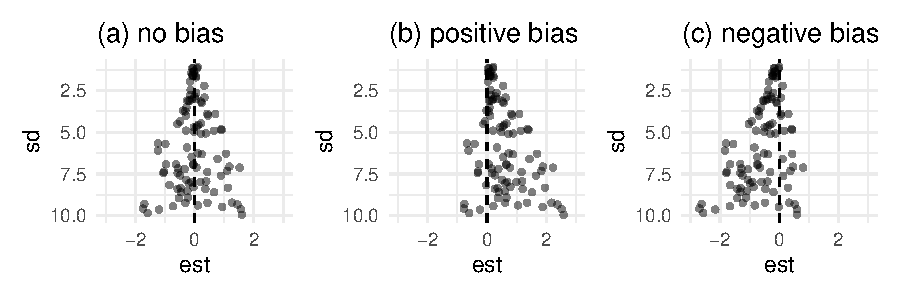
\includegraphics{Draft_RR_files/figure-latex/funnel-plot-1.pdf}
\caption{\label{fig:funnel-plot}Illustrations of funnel plots showing (a) no bias, (b) positive bias, and (c) negative bias in effect sizes. The vertical dashed line represents the meta-analytical mean.}
\end{figure}

\hypertarget{ana-factors}{%
\subsubsection{Analytical and demographic factors affecting effect sizes}\label{ana-factors}}

As a second step, we will investigate (a) the extent to which the individual standardized effect sizes are affected by a series of predictors related to analytical and demographic factors (see below); and (b) the extent to which deviations from the meta-analytical mean by the individual standardized effect sizes relate to those same predictors.
We will fit two Bayesian regression models, one for (a) and one for (b).
with each team's group-level coefficient \(\alpha_{\text{t}[i]}\) as the outcome variable, and the analytical and demographic factors described below as predictors.
The coefficient \(\alpha_{\text{t}[i]}\) can be interpreted as the deviation score of the team's \(\eta_i\) from the meta-analytical mean, allowing us to determine potential effects of analytical and demographic factors on how the teams deviate from the meta-analytical mean.
Since each \(\alpha_{\text{t}[i]}\) comes with uncertainty, quantified by its standard deviation \(\sigma_{\alpha_{\text{t}[i]}}\), we will fit a measurement-error model, as we did in the meta-analytical model above.

A normal distribution will be used as the likelihood of \(\alpha_{t[i]}\).
The mean of \(\alpha_{t[i]}\) is modelled on the basis of the overall intercept \(\beta\) and on the coefficients \(\upsilon_n\) of each predictor.
The numeric predictors will be centered and scaled and the categorical predictors will be sum coded.
As the prior for \(i\) and \(\upsilon\) we will use a normal distribution with mean 0 and standard deviation 1.

\textbf{Analytical factors}. We will model the effect of the following predictors related to the analytical characteristics of each team's reported analysis:

\begin{itemize}
\tightlist
\item
  \emph{Measure of uniqueness} {[}numeric{]} of individual analyses for the set of predictors in each model (\(uniq_i\)).
\item
  \emph{Measure of conservativeness} {[}numeric{]} of the model specification, as the number of random/group-level effects included (\(cons_i\)).
\item
  \emph{Number of post-hoc changes to the acoustic measurements} {[}numeric{]} the teams will report to have carried out (\(phoc_i\)).
\item
  \emph{Number of models} {[}numeric{]} the teams will report to have run (\(modn_i\)).
\item
  \emph{Major dimension} {[}categorical{]} that has been measured to answer the research question (\(mdim_i\)).
\item
  \emph{Temporal window} {[}categorical{]} that the measurement is taken over (\(twin_i\)).
\item
  \emph{Data exclusion}, {[}categorical{]} whether data has been excluded or not (\(excl_i\)).
\item
  \emph{Average peer-review rating} {[}numeric{]}, as the mean of the peer-review ratings for each analysis.
\end{itemize}

The measure of uniqueness of predictors will be assessed by the Sørensen-Dice Index (SDI, Dice 1945; Sørensen 1948).
The SDI is an index typically used in ecology research to compare species composition across sites.
For our purposes, we will treat predictors as species and individual analyses as sites.
For each pair of analyses \((X, Y)\), the SDI will be obtained using the following \highlight[id=SC, comment={refactored the formula so it is closer to the original source}]{formula}:

\[\text{SDI} = \frac{2|X \cap Y|}{|X|+|Y|}\]

where \(|X \cap Y|\) is the number of variables common to both models in the pair, and \(|X|+|Y|\) is the sum of the number of variables that occur in each model.

In order to generate a unique SDI for each analysis team, we will calculate the average of all pairwise SDIs for all pairs of analyses using the \texttt{beta.pair()} function in the betapart R package (Baselga et al. 2020).

The major measurement dimension of each analysis will be categorized according to the following possible groups: \emph{duration}, \emph{amplitude}, \emph{fundamental frequency}, \emph{other spectral properties} (e.g.~frequency center of gravity, harmonics difference, etc.), \emph{other measures} (e.g.~principal components, vowel dispersion, etc.)\comment[id=TR]{Stefano, do you think these four will cover possible ways to measure? We might want to define them too? dunno}\comment[id=SC]{I just added a "other measures" category for other things that are not strictly acoustic.}
The temporal window that the measurement is taken over is defined by the target linguistic unit.
We assume the following relevant linguistic units: \emph{segment}, \emph{syllable}, \emph{word}, \emph{phrase}.
Since each analysis will receive more than one peer-review rating, we will calculate the mean rating and its standard deviation for each.
These will be entered in the model formula with a measurement-error term (\texttt{me(mean,\ sd)} in brms).

\textbf{Demographic factors}. We will include the following demographic factors about the teams:

\begin{itemize}
\tightlist
\item
  \emph{Research experience} {[}numeric{]} as the elapsed time from PhD award. Negative values will indicate that the person is a student or graduate studens (\(rexp_i\)).
\item
  \emph{Initial belief} {[}numeric{]} in the presence of an effect of atypical noun-adjective pairs on acoustics, as answered during the intake questionnaire (\(belf_i\)).
\end{itemize}

We will publicly archive all relevant data, code, and materials on the Open Science Framework (\url{https://osf.io/3bmcp/}).
Archived data will include the original data sets distributed to all analysts, any edited versions of the data analyzed by individual groups, and the data we analyze with our meta-analyses, which include the effect sizes derived from separate analyses, the statistics describing variation in model structure among analysis teams, and the anonymized answers to our surveys of analysts and peer reviewers.
Similarly, we will archive both the analysis code used for each individual analysis and the code from our meta-analyses.
We will also archive copies of our survey instruments from analysts and peer reviewers.

Our rules for excluding data from our study are as follows.
We will exclude from our synthesis any individual analysis submitted after we have completed peer review or those unaccompanied by analysis files that allow us to understand what the analysts did.
We will also exclude any individual analysis that does not produce an outcome that can be interpreted as an answer to our primary question.

\hypertarget{phase-6-collaborative-write-up-of-manuscript}{%
\subsection{Phase 6: Collaborative Write-Up of Manuscript}\label{phase-6-collaborative-write-up-of-manuscript}}

Analysts and initiating authors will discuss the limitations, results, and implications of the study and collaborate on writing the final manuscript for review as a stage-2 Registered Report.

\newpage

\hypertarget{references}{%
\section{References}\label{references}}

\begingroup
\setlength{\parindent}{-0.5in}
\setlength{\leftskip}{0.5in}

\hypertarget{refs}{}
\begin{CSLReferences}{1}{0}
\leavevmode\hypertarget{ref-arts2011overspecification}{}%
Arts, Anja, Alfons Maes, Leo GM Noordman, and Carel Jansen. 2011. {``Overspecification in Written Instruction.''} \emph{Linguistics} 49 (3): 555--74.

\leavevmode\hypertarget{ref-baselga2020}{}%
Baselga, Andres, David Orme, Sebastien Villeger, Julien De Bortoli, Fabien Leprieur, and Maxime Logez. 2020. {``{b}etapart: Partitioning Beta Diversity into Turnover and Nestedness Components.''} \url{https://CRAN.R-project.org/package=betapart}.

\leavevmode\hypertarget{ref-bastiaansen2020}{}%
Bastiaansen, Jojanneke A., Yoram K. Kunkels, Frank J. Blaauw, Steven M. Boker, Eva Ceulemans, Meng Chen, Sy-Miin Chow, et al. 2020. {``Time to Get Personal? The Impact of Researchers Choices on the Selection of Treatment Targets Using the Experience Sampling Methodology.''} \emph{Journal of Psychosomatic Research} 137: 110211.

\leavevmode\hypertarget{ref-botvinik-nezer2020}{}%
Botvinik-Nezer, Rotem, Felix Holzmeister, Colin F. Camerer, Anna Dreber, Juergen Huber, Magnus Johannesson, Michael Kirchler, et al. 2020a. {``Variability in the Analysis of a Single Neuroimaging Dataset by Many Teams.''} \emph{Nature} 582 (7810): 84--88.

\leavevmode\hypertarget{ref-botvinik2020variability}{}%
Botvinik-Nezer, Rotem, Felix Holzmeister, Colin F Camerer, Anna Dreber, Juergen Huber, Magnus Johannesson, Michael Kirchler, et al. 2020b. {``Variability in the Analysis of a Single Neuroimaging Dataset by Many Teams.''} \emph{Nature}, 1--7.

\leavevmode\hypertarget{ref-box1976science}{}%
Box, George EP. 1976. {``Science and Statistics.''} \emph{Journal of the American Statistical Association} 71 (356): 791--99.

\leavevmode\hypertarget{ref-brugger2001}{}%
Brugger, Peter. 2001. {``From Haunted Brain to Haunted Science: A Cognitive Neuroscience View of Paranormal and Pseudoscientific Thought.''} \emph{Hauntings and Poltergeists: Multidisciplinary Perspectives}, January, 195--213.

\leavevmode\hypertarget{ref-burkner2017}{}%
Bürkner, Paul-Christian. 2017. {``{brms}: An {R} Package for {Bayesian} Multilevel Models Using {Stan}.''} \emph{Journal of Statistical Software} 80 (1): 1--28. \url{https://doi.org/10.18637/jss.v080.i01}.

\leavevmode\hypertarget{ref-camerer2018evaluating}{}%
Camerer, Colin F, Anna Dreber, Felix Holzmeister, Teck-Hua Ho, Jürgen Huber, Magnus Johannesson, Michael Kirchler, et al. 2018. {``Evaluating the Replicability of Social Science Experiments in Nature and Science Between 2010 and 2015.''} \emph{Nature Human Behaviour} 2 (9): 637--44. \url{https://doi.org/10.1038/s41562-018-0399-z}.

\leavevmode\hypertarget{ref-de2014thought}{}%
De Groot, Adriaan D. 2014. \emph{Thought and Choice in Chess}. Vol. 4. Walter de Gruyter GmbH \& Co KG.

\leavevmode\hypertarget{ref-degen2020redundancy}{}%
Degen, Judith, Robert D Hawkins, Caroline Graf, Elisa Kreiss, and Noah D Goodman. 2020. {``When Redundancy Is Useful: A Bayesian Approach to {`Overinformative'} Referring Expressions.''} \emph{Psychological Review}.

\leavevmode\hypertarget{ref-dice1945}{}%
Dice, Lee Raymond. 1945. {``Measures of the Amount of Ecologic Association Between Species.''} \emph{Ecology} 26 (3): 297--302.

\leavevmode\hypertarget{ref-dutilh2019}{}%
Dutilh, Gilles, Jeffrey Annis, Scott D. Brown, Peter Cassey, Nathan J. Evans, Raoul Grasman, Guy E. Hawkins, et al. 2019. {``The Quality of Response Time Data Inference: A Blinded, Collaborative Assessment of the Validity of Cognitive Models.''} \emph{Psychonomic Bulletin \& Review} 26 (4): 1051--69.

\leavevmode\hypertarget{ref-egger1997}{}%
Egger, Matthias, George Davey Smith, Martin Schneider, and Christoph Minder. 1997. {``Bias in Meta-Analysis Detected by a Simple, Graphical Test.''} \emph{British Medical Journal} 315: 629--34.

\leavevmode\hypertarget{ref-fischhoff1975hindsight}{}%
Fischhoff, Baruch. 1975. {``Hindsight Is Not Equal to Foresight: The Effect of Outcome Knowledge on Judgment Under Uncertainty.''} \emph{Journal of Experimental Psychology: Human Perception and Performance} 1 (3): 288.

\leavevmode\hypertarget{ref-flake2020}{}%
Flake, Jessica Kay, and Eiko I. Fried. 2020. {``Measurement Schmeasurement: Questionable Measurement Practices and How to Avoid Them.''} \emph{Advances in Methods and Practices in Psychological Science} 3 (4): 456--65. \url{https://doi.org/10.1177/2515245920952393}.

\leavevmode\hypertarget{ref-foulkes2006}{}%
Foulkes, Paul, and Gerard Docherty. 2006. {``The Social Life of Phonetics and Phonology.''} \emph{Journal of Phonetics} 34 (4): 409--38.

\leavevmode\hypertarget{ref-gatt2013we}{}%
Gatt, Albert, Roger PG van Gompel, Kees van Deemter, and Emiel Krahmer. 2013. {``Are We Bayesian Referring Expression Generators.''} In. Cognitive Science Society.

\leavevmode\hypertarget{ref-gelman2014statistical}{}%
Gelman, Andrew, and Eric Loken. 2014. {``The Statistical Crisis in Science: Data-Dependent Analysis--a" Garden of Forking Paths"--Explains Why Many Statistically Significant Comparisons Don't Hold Up.''} \emph{American Scientist} 102 (6): 460--66.

\leavevmode\hypertarget{ref-gordon2017acoustic}{}%
Gordon, Matthew, and Timo Roettger. 2017. {``Acoustic Correlates of Word Stress: A Cross-Linguistic Survey.''} \emph{Linguistics Vanguard} 3 (1): 1--11.

\leavevmode\hypertarget{ref-grice1975logic}{}%
Grice, Herbert P. 1975. {``Logic and Conversation.''} In \emph{Speech Acts}, 41--58. Brill.

\leavevmode\hypertarget{ref-hawkins2004influence}{}%
Hawkins, Sarah, and Noël Nguyen. 2004. {``Influence of Syllable-Coda Voicing on the Acoustic Properties of Syllable-Onset /l/ in {E}nglish.''} \emph{Journal of Phonetics} 32 (2): 199--231.

\leavevmode\hypertarget{ref-jongman2000acoustic}{}%
Jongman, Allard, Ratree Wayland, and Serena Wong. 2000. {``Acoustic Characteristics of English Fricatives.''} \emph{The Journal of the Acoustical Society of America} 108 (3): 1252--63.

\leavevmode\hypertarget{ref-knight2000}{}%
Knight, K. 2000. \emph{Mathematical Statistics}. Chapman; Hall, New York.

\leavevmode\hypertarget{ref-koole2012rewarding}{}%
Koole, Sander L, and Daniël Lakens. 2012. {``Rewarding Replications: A Sure and Simple Way to Improve Psychological Science.''} \emph{Perspectives on Psychological Science} 7 (6): 608--14.

\leavevmode\hypertarget{ref-ladd2008intonational}{}%
Ladd, D Robert. 2008. \emph{Intonational Phonology}. Cambridge University Press.

\leavevmode\hypertarget{ref-lau2006}{}%
Lau, Joseph, John P. A. Ioannidis, Norma Terrin, Christopher H. Schmid, and Ingram Olkin. 2006. {``The Case of the Misleading Funnel Plot.''} \emph{British Medical Journal} 333 (7568): 597--600.

\leavevmode\hypertarget{ref-light1984}{}%
Light, Richard J., and David B. Pillemer. 1984. \emph{Summing up; the Science of Reviewing Research}. Cambridge, MA (USA) Harvard Univ. Press.

\leavevmode\hypertarget{ref-lisker1977rapid}{}%
Lisker, Leigh. 1977. {``Rapid Versus Rabid: A Catalogue of Acoustic Features That May Cue the Distinction.''} \emph{The Journal of the Acoustical Society of America} 62 (S1): S77--78.

\leavevmode\hypertarget{ref-lisker1986voicing}{}%
---------. 1986. {``{`Voicing'} in {E}nglish: A Catalogue of Acoustic Features Signaling /b/ Versus /p/ in Trochees.''} \emph{Language and Speech} 29 (1): 3--11.

\leavevmode\hypertarget{ref-nickerson1998confirmation}{}%
Nickerson, Raymond S. 1998. {``Confirmation Bias: A Ubiquitous Phenomenon in Many Guises.''} \emph{Review of General Psychology} 2 (2): 175--220.

\leavevmode\hypertarget{ref-nosek2014method}{}%
Nosek, Brian A, and Daniël Lakens. 2014. {``A Method to Increase the Credibility of Published Results.''} \emph{Social Psychology} 45 (3): 137--41.

\leavevmode\hypertarget{ref-ogden2004}{}%
Ogden, Richard. 2004. {``Non-Modal Voice Quality and Turn-Taking in {F}innish.''} \emph{Sound Patterns in Interaction: Cross-Linguistic Studies from Conversation}, 29--62.

\leavevmode\hypertarget{ref-open2015estimating}{}%
Open Science Collaboration. 2015. {``Estimating the Reproducibility of Psychological Science.''} \emph{Science} 349 (6251). \url{https://doi.org/10.1126/science.aac4716}.

\leavevmode\hypertarget{ref-paraboni2007generating}{}%
Paraboni, Ivandré, Kees Van Deemter, and Judith Masthoff. 2007. {``Generating Referring Expressions: Making Referents Easy to Identify.''} \emph{Computational Linguistics} 33 (2): 229--54.

\leavevmode\hypertarget{ref-R-base}{}%
R Core Team. 2020. \emph{R: A Language and Environment for Statistical Computing}. Vienna, Austria: R Foundation for Statistical Computing. \url{https://www.R-project.org/}.

\leavevmode\hypertarget{ref-roettger2019researcher}{}%
Roettger, Timo B. 2019. {``Researcher Degrees of Freedom in Phonetic Research.''} \emph{Laboratory Phonology: Journal of the Association for Laboratory Phonology} 10 (1).

\leavevmode\hypertarget{ref-rotello2015more}{}%
Rotello, Caren M, Evan Heit, and Chad Dubé. 2015. {``When More Data Steer Us Wrong: {R}eplications with the Wrong Dependent Measure Perpetuate Erroneous Conclusions.''} \emph{Psychonomic Bulletin \& Review} 22 (4): 944--54.

\leavevmode\hypertarget{ref-rubio2016redundant}{}%
Rubio-Fernández, Paula. 2016. {``How Redundant Are Redundant Color Adjectives? An Efficiency-Based Analysis of Color Overspecification.''} \emph{Frontiers in Psychology} 7: 153.

\leavevmode\hypertarget{ref-sedivy2003pragmatic}{}%
Sedivy, Julie C. 2003. {``Pragmatic Versus Form-Based Accounts of Referential Contrast: Evidence for Effects of Informativity Expectations.''} \emph{Journal of Psycholinguistic Research} 32 (1): 3--23.

\leavevmode\hypertarget{ref-silberzahn2018many}{}%
Silberzahn, Raphael, Eric Luis Uhlmann, Daniel P Martin, Pasquale Anselmi, Frederik Aust, Eli Awtrey, Štěpán Bahnı́k, et al. 2018. {``Many Analysts, One Data Set: Making Transparent How Variations in Analytic Choices Affect Results.''} \emph{Advances in Methods and Practices in Psychological Science} 1 (3): 337--56.

\leavevmode\hypertarget{ref-simmons2011false}{}%
Simmons, Joseph P, Leif D Nelson, and Uri Simonsohn. 2011. {``False-Positive Psychology: Undisclosed Flexibility in Data Collection and Analysis Allows Presenting Anything as Significant.''} \emph{Psychological Science} 22 (11): 1359--66.

\leavevmode\hypertarget{ref-stan2020a}{}%
Stan Development Team. 2020. {``{RStan}: The {R} Interface to {Stan}.''} \url{http://mc-stan.org/}.

\leavevmode\hypertarget{ref-stan2021}{}%
---------. 2021. {``Stan Modeling Language Users Guide and Reference Manual, V2.26.0.''} \url{http://mc-stan.org/}.

\leavevmode\hypertarget{ref-starns2019}{}%
Starns, Jeffrey J., Andrea M. Cataldo, Caren M. Rotello, Jeffrey Annis, Andrew Aschenbrenner, Arndt Bröder, Gregory Cox, et al. 2019a. {``Assessing Theoretical Conclusions with Blinded Inference to Investigate a Potential Inference Crisis.''} \emph{Advances in Methods and Practices in Psychological Science} 2 (4): 335--49.

\leavevmode\hypertarget{ref-starns2019assessing}{}%
Starns, Jeffrey J, Andrea M Cataldo, Caren M Rotello, Jeffrey Annis, Andrew Aschenbrenner, Arndt Bröder, Gregory Cox, et al. 2019b. {``Assessing Theoretical Conclusions with Blinded Inference to Investigate a Potential Inference Crisis.''} \emph{Advances in Methods and Practices in Psychological Science} 2 (4): 335--49.

\leavevmode\hypertarget{ref-sterling1959publication}{}%
Sterling, Theodore D. 1959. {``Publication Decisions and Their Possible Effects on Inferences Drawn from Tests of Significance--or Vice Versa.''} \emph{Journal of the American Statistical Association} 54 (285): 30--34.

\leavevmode\hypertarget{ref-sterne2005}{}%
Sterne, Jonathan A. C., Betsy Jane Becker, and Matthias Egger. 2005. {``The Funnel Plot.''} In \emph{Publication Bias in Meta-Analysis: Prevention, Assessment and Adjustments}, edited by Hannah R. Rothstein, Alexander J. Sutton, and Michael Borenstein, 75--98. Wiley Online Library.

\leavevmode\hypertarget{ref-sorensen1948}{}%
Sørensen, Thorlvald. 1948. {``A Method of Establishing Groups of Equal Amplitude in Plant Sociology Based on Similarity of Species and Its Application to Analyses of the Vegetation on {D}anish Commons.''} \emph{Kongelige Danske Videnskabernes Selskab} 5 (4): 1--34.

\leavevmode\hypertarget{ref-tukey1977exploratory}{}%
Tukey, John W. 1977. \emph{Exploratory Data Analysis}. Vol. 2. Reading, MA.

\leavevmode\hypertarget{ref-tversky1974judgment}{}%
Tversky, Amos, and Daniel Kahneman. 1974. {``Judgment Under Uncertainty: Heuristics and Biases.''} \emph{Science} 185 (4157): 1124--31.

\leavevmode\hypertarget{ref-heuven2002}{}%
Van Heuven, Vincent J, Judith Haan, Carlos Gussenhoven, and Natasha Warner. 2002. {``Temporal Distribution of Interrogativity Markers in {D}utch: A Perceptual Study.''} In \emph{Laboratory Phonology 7}, 4:61. 1. Walter de Gruyter.

\leavevmode\hypertarget{ref-van2005speech}{}%
Van Heuven, Vincent J, and Ellen Van Zanten. 2005. {``Speech Rate as a Secondary Prosodic Characteristic of Polarity Questions in Three Languages.''} \emph{Speech Communication} 47 (1-2): 87--99.

\leavevmode\hypertarget{ref-wagenmakers2012agenda}{}%
Wagenmakers, Eric-Jan, Ruud Wetzels, Denny Borsboom, Han LJ van der Maas, and Rogier A Kievit. 2012. {``An Agenda for Purely Confirmatory Research.''} \emph{Perspectives on Psychological Science} 7 (6): 632--38.

\leavevmode\hypertarget{ref-westerbeek2015stored}{}%
Westerbeek, Hans, Ruud Koolen, and Alfons Maes. 2015. {``Stored Object Knowledge and the Production of Referring Expressions: The Case of Color Typicality.''} \emph{Frontiers in Psychology} 6: 935.

\leavevmode\hypertarget{ref-white2009}{}%
White, Laurence, Elinor Payne, and Sven L. Mattys. 2009. {``Rhythmic and Prosodic Contrast in {V}enetan and {S}icilian {I}talian.''} In \emph{Phonetics and Phonology: Interactions and Interrelations}, edited by M. Vigario, S. Frota, and M. J. Freitas, 137--58. Amsterdam: John Benjamins.

\leavevmode\hypertarget{ref-wicherts2016}{}%
Wicherts, Jelte M., Coosje L. S. Veldkamp, Hilde E. M. Augusteijn, Marjan Bakker, Robbie C. M. van Aert, and Marcel A. L. M. van Assen. 2016. {``Degrees of Freedom in Planning, Running, Analyzing, and Reporting Psychological Studies: A Checklist to Avoid p-Hacking.''} \emph{Frontiers in Psychology} 7. \url{https://doi.org/10.3389/fpsyg.2016.01832}.

\leavevmode\hypertarget{ref-wicherts2006poor}{}%
Wicherts, Jelte M, Denny Borsboom, Judith Kats, and Dylan Molenaar. 2006. {``The Poor Availability of Psychological Research Data for Reanalysis.''} \emph{American Psychologist} 61 (7): 726.

\leavevmode\hypertarget{ref-winter2014spoken}{}%
Winter, Bodo. 2014. {``Spoken Language Achieves Robustness and Evolvability by Exploiting Degeneracy and Neutrality.''} \emph{BioEssays} 36 (10): 960--67.

\end{CSLReferences}

\endgroup

\end{document}
